\documentclass[a4paper, 11pt]{article} % for final document
% \documentclass[draft, a4paper,11pt]{article} % for drafts

\usepackage{geometry} % for impagination
\geometry{
     left=20mm,
     right=20mm,
     top=25mm
 }

\usepackage{graphicx} % Required for inserting images
\usepackage[utf8]{inputenc}
\usepackage{amsmath}
\usepackage[parfill]{parskip}
\usepackage{float}
\usepackage{subfigure}
\usepackage{svg}
\usepackage[bookmarks]{hyperref}
\usepackage{caption}
\hypersetup{
    colorlinks=true,
    urlcolor=blue
}
\usepackage{microtype} % improves line filling [raccomended]
\usepackage{listings} % highlights code
\usepackage{bookmark} %improve bookmarks
\usepackage[english]{babel} % language
\usepackage[english]{varioref} % for relative reference (vref)
\usepackage[justification=centering]{caption} % for centering the captions
\usepackage{fancyvrb} % for better verbatim
\usepackage{multicol} % for multicolumns
\setlength{\columnsep}{1cm}

% Configure bibliography
\usepackage[backend=biber]{biblatex}
\addbibresource{references.bib}
\AtBeginBibliography{\footnotesize} % make text smaller for bibliography


\title{\textbf{Indoor navigation assistant for visually impaired people}}
\author{Salvatore Lombardi \\ \href{mailto:s.lombardi38@studenti.unipi.it}{s.lombardi38@studenti.unipi.it} \and Francesco Martoccia \\ \href{mailto:s.lombardi38@studenti.unipi.it}{f.martoccia@studenti.unipi.it} \and Riccardo Sagramoni \\ \href{mailto:s.lombardi38@studenti.unipi.it}{r.sagramoni@studenti.unipi.it} \and Luca Tartaglia \\ \href{mailto:s.lombardi38@studenti.unipi.it}{l.tartaglia@studenti.unipi.it}}
\date{}

\begin{document}

\maketitle

\begin{multicols*}{2}

\section{Abstract}

Indoor-assisted navigation presents a significant challenge for individuals who are blind or visually impaired \cite{9126068, MURATA201914, en12193702, s20030636}.
The limitations of traditional location technologies, such as GPS tracking, prevent achieving the necessary accuracy within enclosed buildings \cite{RAZAVI2012128, localization-taxonomy}.
Accurate indoor navigation is vital for people with visual impairments, as it empowers them to navigate unfamiliar indoor environments independently and safely \cite{9126068}.

To achieve an indoor navigation assistant tailored for enclosed buildings we employed a hybrid approach, combining two different technologies known for their success in similar contexts \cite{MURATA201914, s20030636}: 
a network of \textbf{Bluetooth Low Energy beacons}, which allowed us to localize the user inside a \textit{region} within the building \cite{localization-taxonomy, 10.1145/3058555.3058560, en12193702}, and \textbf{QR codes}, which can inform the application about the presence of points of interest around the user \cite{indoor-navigation-qr-codes}.

Once the application was developed, we proceeded to instrument a section of the main building at the \textit{School of Engineering, University of Pisa}, by strategically placing BLE beacons and QR codes along the hallway.

The results we obtained were quite satisfactory. The application successfully guided the users along the designated path, being able to detect region switches, nearby points of interests and incoming curves with a good level of accuracy and responsiveness.

\section{Introduction}

The goal of the application is to provide help to people with visual impairments in navigating indoor environments, such as universities, hospitals, or other places where technologies like GPS location prove inaccurate. Very often, finding one's way around enclosed facilities, especially large ones, can be difficult for people with this type of disability. For this reason, the application aims to constantly provide, through voice support, information about the areas where the person is located and the related points of interest.

To achieve the described goal, it was decided to adopt an approach based on Bluetooth Low Energy beacons and QR codes.
After the development of the application, a specific section of the main building of the School of Engineering at the University of Pisa was chosen to conduct the associated tests. A network of beacons (from \textit{Kontakt.io} \cite{kontakt:beacons}), placed at a certain distance from each other, was then created to divide the environment considered for the experiments into regions. Each area, identified by the application by exploiting the RSSI values associated with the beacons' signals, was equipped with QR codes corresponding to the possible points of interest in it. The user, walking within the test area, is updated, via \textit{Text-to-Speech technology} \cite{android:text-to-speech-ref}, about the region he or she is in. In addition, by framing the QR codes he can pinpoint the exact location of a classroom or bathroom, for example (thanks to the \textit{ML Kit library}, provided by Google \cite{android:mlkit:overview}). Moreover, when encountering a curved section, the application can promptly notify the user and offer them the necessary directions. 

The rest of the paper is organized as follows: Section \vref{sec:architecture} presents the system architecture, Section \vref{sec:experimental_results} shows the experimental results and in Section \vref{sec:conclusion} the conclusions are drawn.

\section{Architecture}
\label{sec:architecture}

\subsection{Application activities}
There are two major activities used in the development of the application: the Main Activity and the Navigation Activity.

The \textbf{Main Activity} displays the menu page, where the user can find a brief description of the application. By tapping the "Go to Navigation" button the user can access the navigation page. This activity is responsible for initializing the necessary dependencies of the Kontatk SDK (BLE beacon API) and managing Bluetooth and Camera Permissions. It checks if the permissions are enabled and prompts the user to activate them if needed.

The \textbf{Navigation Activity} serves as the core part of the application. Its primary responsibility is to enable and verify Bluetooth and GPS Location services.
Subsequently, it instantiates the BLE beacons and QR Code scanners to provide localization and navigation functionalities to the user. As part of its debugging mode, this activity displays updated information about the current region detected and the points of interest (BLE Beacon functionalities). It also shows the updated QR Code point of interest scanned (QR Code functionality). Furthermore, it includes a button to activate the camera view on the screen.

\vfill\null
\columnbreak

\begin{figure}[H]
    \centering
    \begin{subfigure}
        \centering
        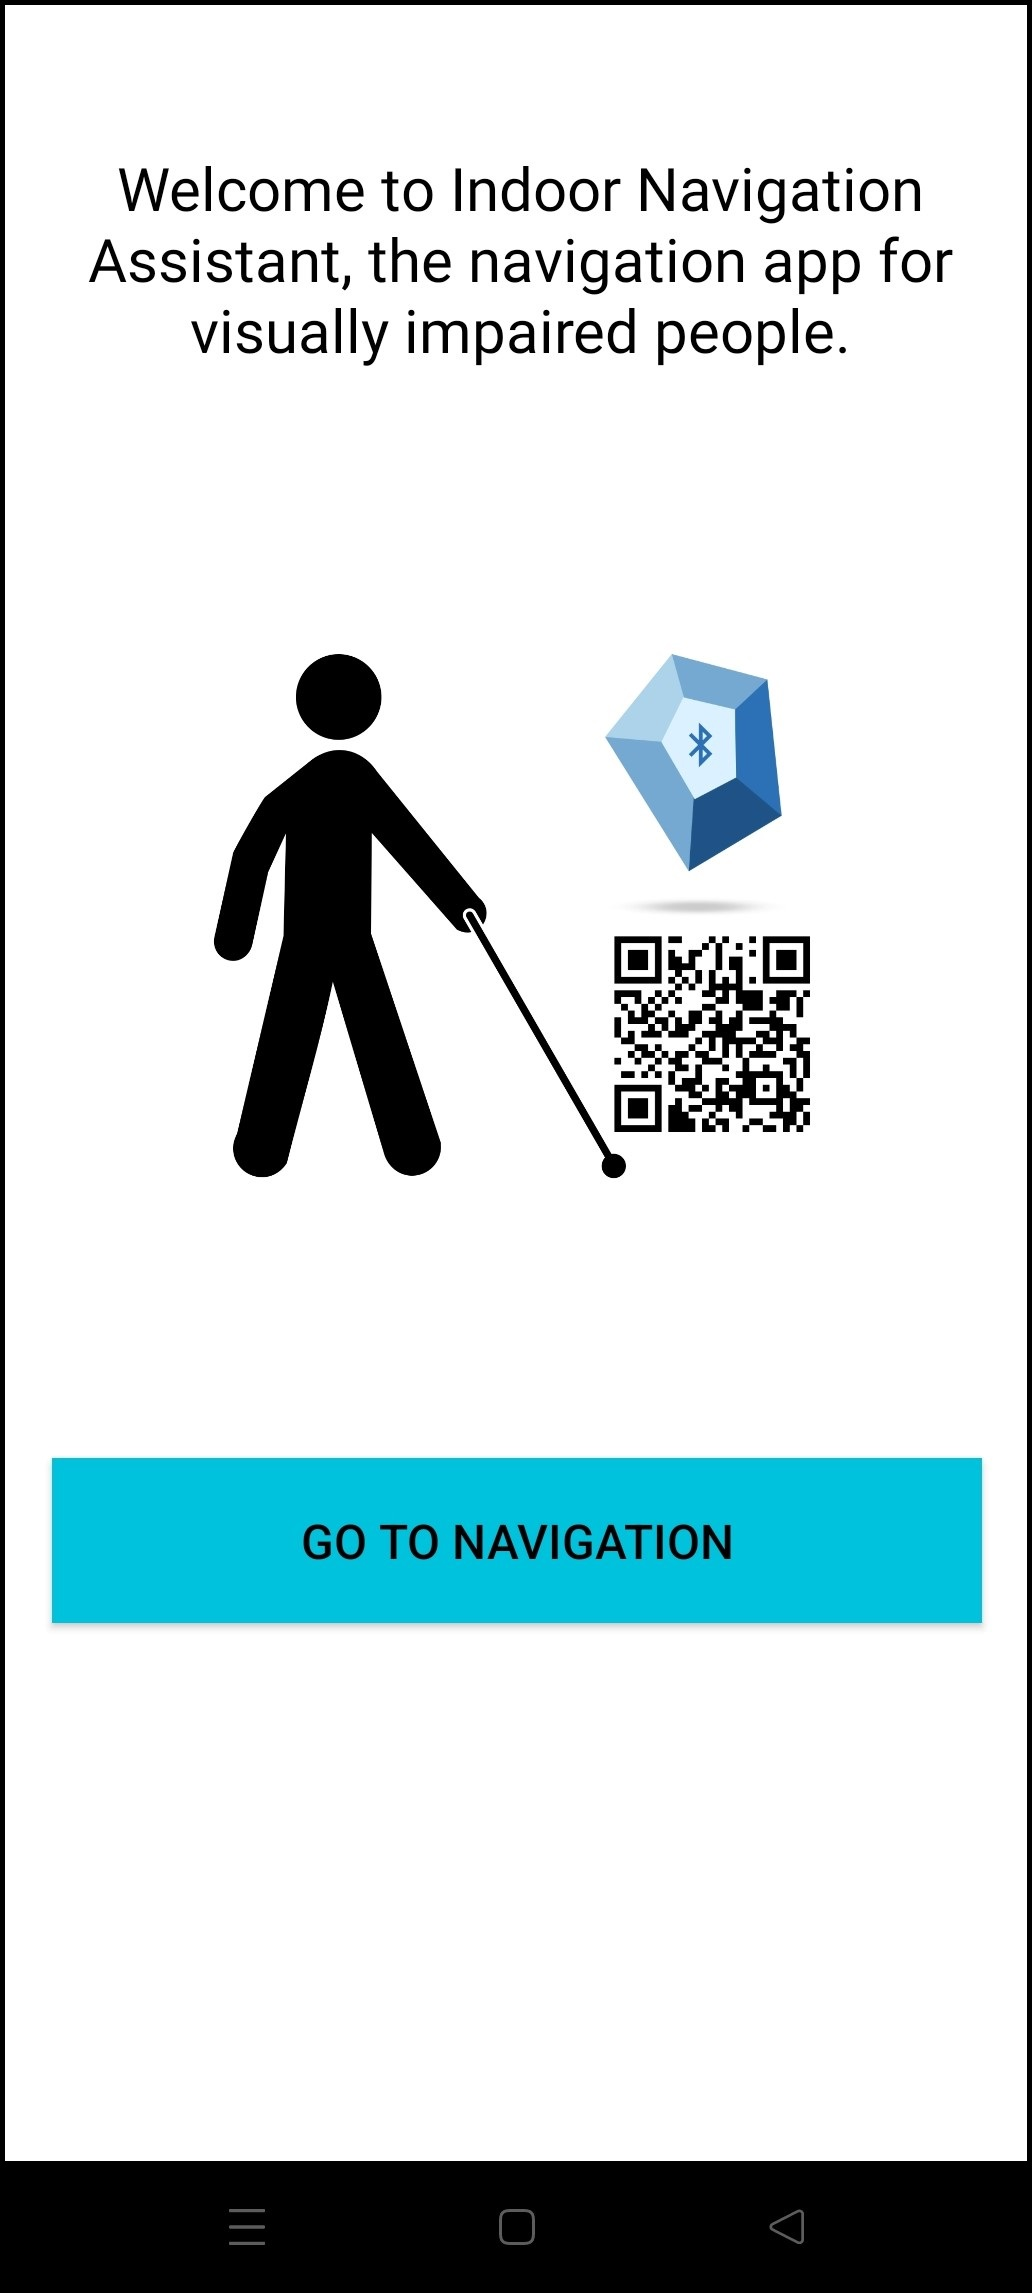
\includegraphics[width=0.2\textwidth]{chapters/architecture/images/main_activity.jpg}
        \label{fig:my_label}
    \end{subfigure}
    \hfill
    \begin{subfigure}
        \centering
        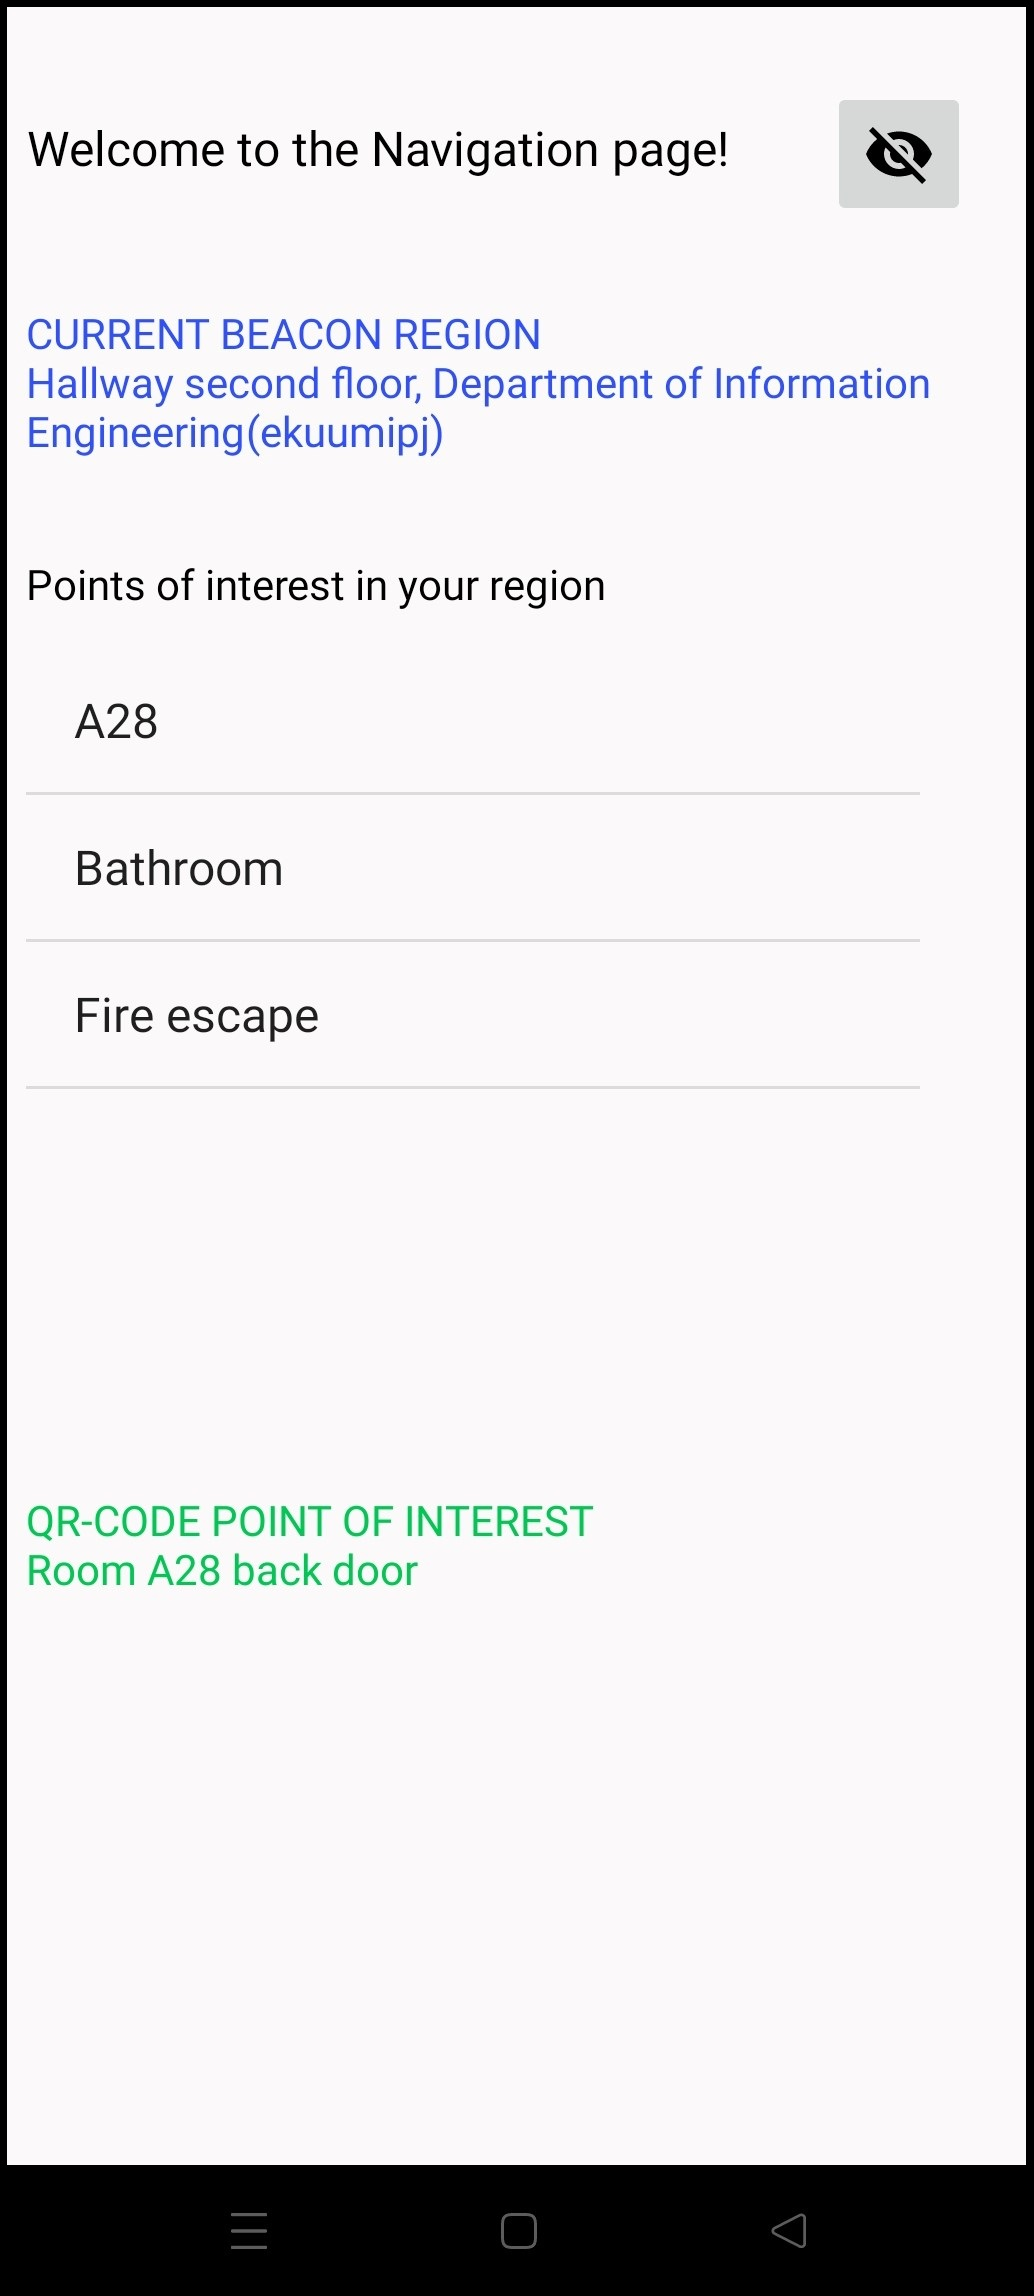
\includegraphics[width=0.2\textwidth]{chapters/architecture/images/navigation_activity.jpg}
    \end{subfigure}
    \caption{Main Activity and Navigation Activity Pages}
\end{figure}


\subsection{BLE Beacons}
\textbf{Bluetooth Low Energy (BLE) Beacon} technology was utilized to accurately determine the user's location and provide them with relevant information regarding their current region and nearby points of interest. Furthermore, it was employed to notify the user if they are approaching a curve and indicate the appropriate direction to follow.

For this purpose was used the SDK provided directly by the beacon manufacturer and, through the information obtained with the latter, a localization logic was implemented, which was called \textbf{"region-based localization"}.

\begin{figure}[H]
    \centering
    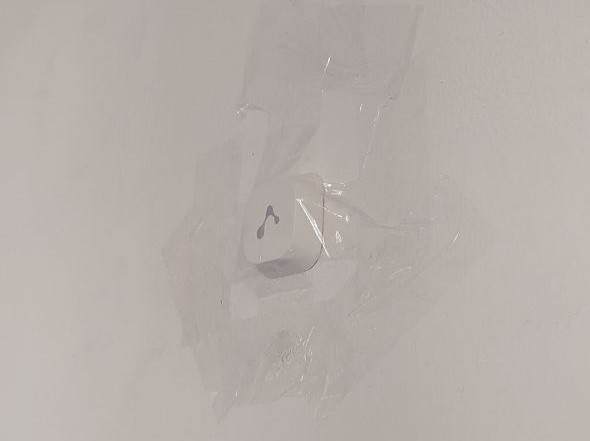
\includegraphics[scale=0.4]{chapters/architecture/images/beacon.jpg}
    \caption{Example of Kontakt iBeacon used to instrument the environment}
\end{figure}


\subsubsection{Kontakt SDK}
The SDK provided by \textbf{kontakt.io} was used to develop the Android application, integrating the localization logic for beacons through the methods it provides. \cite{kontakt:sdk}

Through the use of the \textbf{Proximity Manager}, a high-level component that allows to set the configuration information and scanning the devices, it was possible to receive information from the beacons. 
In particular, this component was able to provide information regarding newly discovered beacons and the signal update of already scanned beacons, returning the information needed to implement the localization logic, such as the \textbf{IDs} of the scanned beacons and their \textbf{Received Signal Strength Indicator (RSSI)}.


\subsubsection{Region-Based Localization\\ Method}
The \textbf{localization method} developed using BLE beacons divides the areas into regions, which are defined by the two beacons with the highest RSSI values.

The initial step entails uploading JSON files containing the required information regarding regions, points of interest, and curves. Moreover, the system consistently listens for incoming data from the beacons, extracting their IDs and RSSI values.

Whenever information is received from newly discovered or updated beacons, the system performs a check to determine if the two beacons with the highest power levels can form a new region. If the IDs of these beacons do not correspond to an existing region, the check is then extended to the next set of beacons. This process continues, iterating through all possible combinations of the three beacons with the highest power levels. By doing so, the search for a new region is optimized, ensuring that false positives are not created.

The transition from one region to another is determined by a predefined threshold. For a region to be recognized as the current region, it must be scanned a minimum number of times equal to the threshold value. Once the threshold is reached, the system considers the new region as the current one and triggers the transition accordingly. Whenever a region change occurs, the user is promptly notified of the current region, this notification includes a list of points of interest that are located within the newly identified region.

During region transitions, it is possible for a region to be identified as a \textbf{pre-curve} or a \textbf{curve}. When a region change occurs, the system checks if the current region is a pre-curve. If it is, the pre-curve ID is saved for future reference. On the other hand, if the current region is a curve, the system notifies the user about the upcoming turn. By utilizing the previously saved pre-curve ID, the system is able to determine the appropriate direction for the user to navigate while approaching the curve. This functionality ensures that the user receives timely alerts and guidance for navigating through curves and pre-curves.

\vspace{3mm}
\begin{figure}[H]
    \centering
    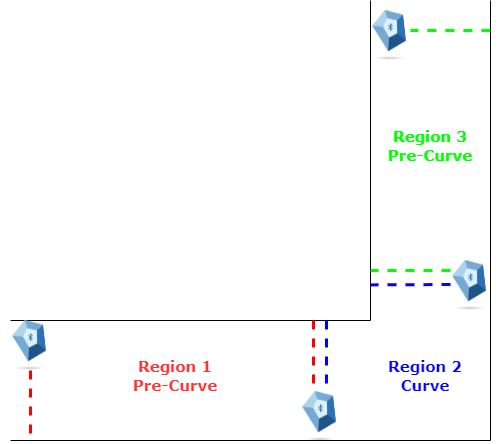
\includegraphics[width=0.9\columnwidth]{chapters/architecture/images/ble_beacons_regions.png}
    \caption{Example of environment region-based division delimited by 2 beacons}
\end{figure}


\subsection{QR codes}
QR codes technology has been employed to identify distincts \textbf{points of interest (POIs)} within the indoor environment. \textit{POIs} represent specific locations that the users may find useful or interesting, such as bathrooms or lecture rooms.

To implement our application effectively, we have utilized two types of QR codes: \textit{floor} QR codes and \textit{door} QR codes. The \textit{floor} QR codes have been positioned on the ground in front of each POI, allowing users to scan them while walking. On the other hand, the \textit{door} QR codes have been placed on the doors of the respective POIs. These QR codes serve as markers for users to easily find the wanted POI.

For this purpose, we adopted the CameraX API for handling the camera and Google's ML Kit API for analyzing the taken images.


\subsubsection{CameraX and ML Kit}

\textbf{CameraX} is an Android Jetpack library, built to help make camera app development easier. 
It provides a consistent, easy-to-use API that works across the vast majority of Android devices.\cite{android:camerax:overview}
One of the main strengths of CameraX is its ease of use: in fact, the API emphasizes \textit{use cases}, which allows the developer to focus on the task that needs to be done instead of managing device-specific nuances.\cite{android:camerax:analyze}
In particular, CameraX offers a pre-built \textit{Image Analysis} use case, which provides CPU-accessible buffers on which can be performed image processing, computer vision, or machine learning inference.\cite{android:camerax:analyze}

\textbf{ML Kit} is a mobile SDK (Software Development Kit) provided by Google that enables developers to integrate\textit{ machine learning capabilities} into their Android and iOS applications. 
ML Kit offers a range of ready-to-use APIs and pre-trained models, simplifying the process of incorporating machine learning functionality into mobile apps without requiring extensive machine learning expertise.\cite{android:mlkit:overview}

In particular, ML Kit offers a \textbf{barcode scanning API}, which allows the developer to read data encoded using most standard barcode formats, such as \textit{QR codes}.\cite{android:mlkit:barcode}
Its key capabilities are the following:
\begin{itemize}
    \item Out-of-the-box support for \textit{most standard barcode formats}, both linear and 2D.
    \item Automatic \textit{format detection}.
    \item Automatically parses \textit{structured data} stored in the barcode.
    \item Recognizes and scans barcodes regardless their \textit{orientation}.
    \item Runs locally on the \textit{device}.
\end{itemize}

Android offers a library (\path{androidx.camera.mlkit.vision}) which provides a \textbf{seamless integration} between CameraX and Google's ML Kit\cite{androidx.camera.mlkit.vision}, which allows to directly forward frames generated in the \textit{Image Analysis} use case to the \textit{barcode scanner}.\cite{androidx.camera.mlkit.vision.MlKitAnalyzer}



\subsubsection{QR codes deployment}

As mentioned earlier, we implemented two distinct types of QR codes: floor QR codes and door QR codes.

The application utilizes \textbf{floor QR codes} to alert users about nearby points of interest. 
To ensure that QR codes are not missed by the walking user, we decided to position \textit{horizontal strips} of QR codes across the entire width of the hallway, as shown in Figure \vref{fig:floor-qr-codes}. 
This design choice is inspired by the \textit{NavCog system}\cite{indoor-navigation-qr-codes}, which achieved error-free scanning of QR codes for indoor navigation.

\begin{figure}[H]
    \centering
    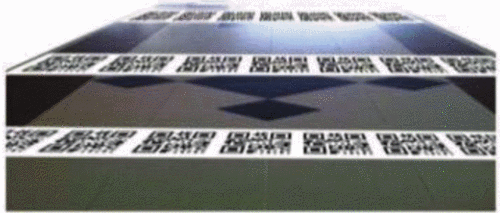
\includegraphics[width=\columnwidth]{chapters/architecture/images/ground-qr-codes.png}
    \caption{Example of intended arrangement of QR codes placed on the ground.\cite{indoor-navigation-qr-codes}}
    \label{fig:floor-qr-codes}
\end{figure}

To ensure effective scanning, the user is required to hold their smartphone device \textit{horizontally} and direct the camera towards the ground. Once the application successfully scans a QR code on the floor, it immediately provides an audible notification to inform the user about the nearby presence of the corresponding point of interest.

As depicted in Figure \vref{fig:multiple-qr-codes}, Google's ML Kit library effectively distinguishes between \textit{different QR codes} within the same image frame. 
Our application is designed to analyze and process \textit{only one of the detected QR codes at a time}, so, since the QR codes in the same strip contain the same value, the presence of multiple QR codes in close proximity will not cause any interference or confusion in its functionality.


\begin{figure}[H]
    \centering
    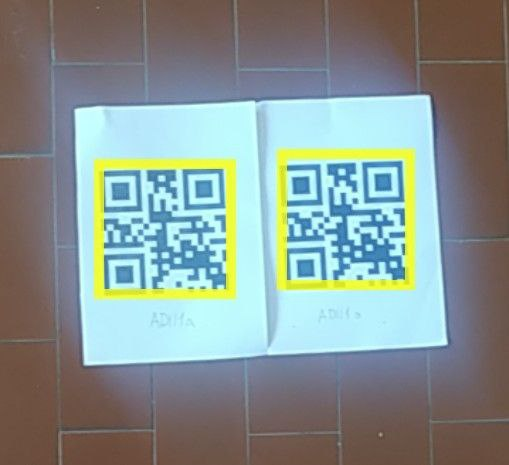
\includegraphics[width=0.6\columnwidth]{chapters/architecture/images/multiple-qr-codes.jpg}
    \caption{Screenshot taken from the Android app which shows how the ML Kit library is able to discern different QR codes in the same frame.}
    \label{fig:multiple-qr-codes}
\end{figure}


On the other hand, the \textbf{door QR codes} are employed to specify the \textit{exact} location of a point of interest (Figure \vref{fig:door-qr-codes}). Once the user locates the relevant floor QR code, which indicates the nearby presence of the point of interest, they should hold their smartphone in a \textit{vertical} position, so that the application can scan the surrounding environment and determine the precise direction in which the point of interest is situated.


\begin{figure}[H]
    \centering
    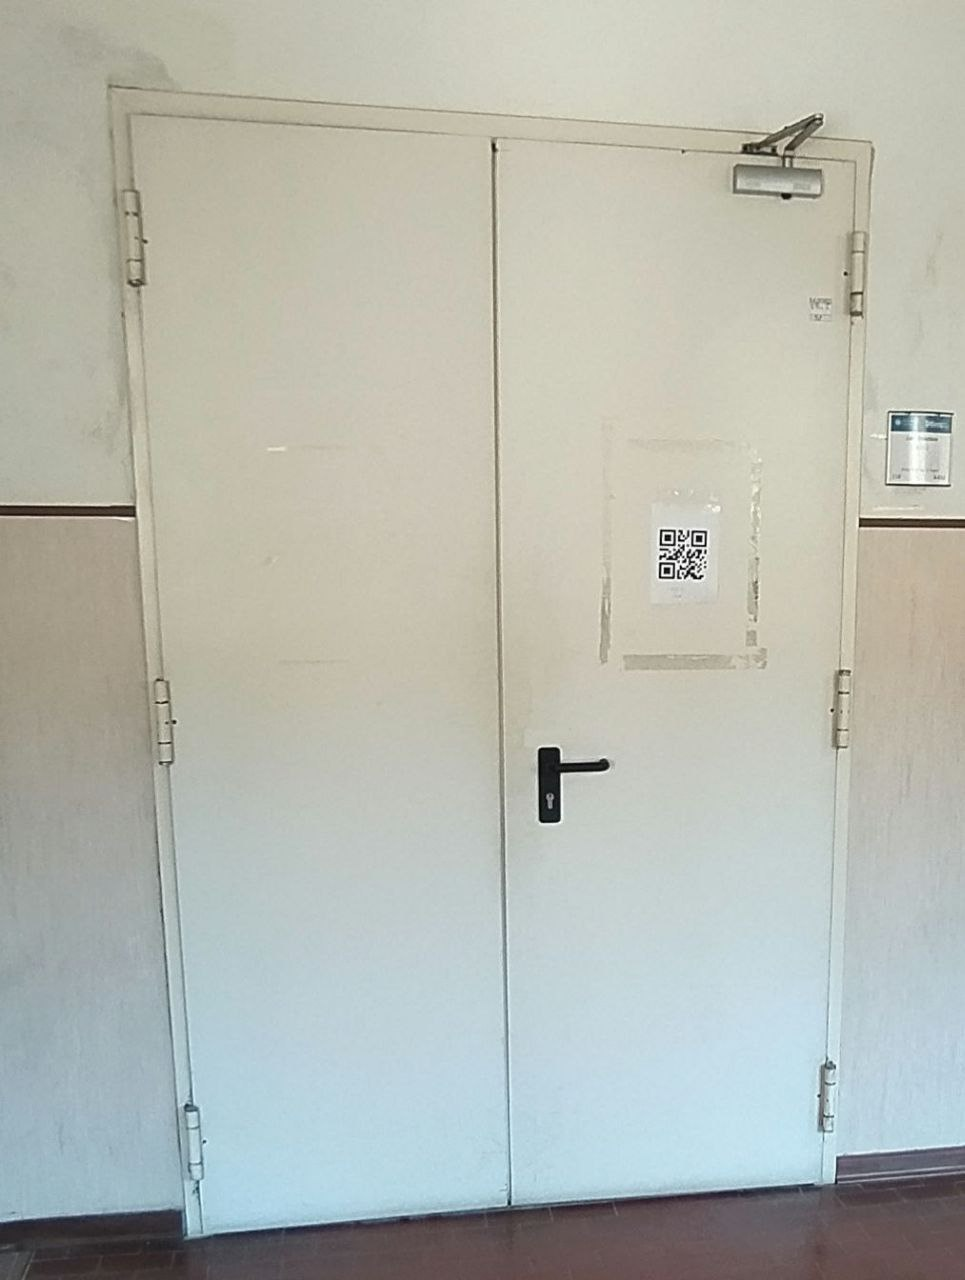
\includegraphics[width=0.6\columnwidth]{chapters/architecture/images/door-qr-codes.jpg}
    \caption{Example of intended arrangement of QR codes placed directly on the points of interest (a door, in this case).}
    \label{fig:door-qr-codes}
\end{figure}


\subsection{Accessibility}
Since our application specifically targets \textit{visually impaired users}, every interaction has been designed to be vocal, rather than written. 
To achieve this, we employed two different technologies: \textit{Talkback} and \textit{TextToSpeech}.


\textbf{Talkback} is a native Android functionality which \textit{announces content through a synthesized voice} and \textit{performs actions on an app in response to user gestures}\cite{android:accessibility}. 
In our application, it plays a crucial role in assisting users in pressing the button to start the navigation activity, granting required Android permissions, and enabling GPS and Bluetooth services.\cite{android:request-runtime-permissions, android:bluetooth-setup}


\textbf{TextToSpeech} is a functionality provided by the \texttt{android.speech.tts} library which \textit{synthesizes speech from a text for immediate playback}.\cite{android:text-to-speech-ref}
This feature is crucial for announcing navigation directions and the presence of nearby points of interest. 

The TextToSpeech object maintains a \textit{First-In-First-Out} (FIFO) queue of texts to be spoken, offering two queuing modes: \texttt{QUEUE\_ADD}, which appends new text to the existing queue, and \texttt{QUEUE\_FLUSH}, which clears the current queue before appending the new text.

In our application, we have adopted the \texttt{QUEUE\_FLUSH} mode for high-priority announcements, such as approaching turns or nearby points of interest. On the other hand, the \texttt{QUEUE\_ADD} mode has been utilized for low-priority announcements, such as region announcements. 
This ensures that important information takes precedence, enhancing the user's navigation experience.


\section{Experimental Results}
\label{sec:experimental_results}
To properly analyze the behavior of the application, numerous tests were conducted within a section of the second floor of the main building of the School of Engineering of the University of Pisa, which has been set with the elements needed for this purpose.

\subsection{Environment\\ instrumentation}
The test environment considered is characterized by three corridors, divided by two curves, and has the following points of interest: the ADII classroom, the A28 classroom, a bathroom, a fire escape, an elevator, and a meeting room. To conduct the experiment and allow the algorithm implemented in the application to function correctly, several attempts were made to arrange the beacons in the considered section. 

In the final setting of the area, the beacons were placed at a distance of about 8 meters from each other and, in zones representing curves, they were placed at a slightly shorter distance to let the application be as responsive as possible in alerting the user of the presence of these particular regions. To permit easy identification of the points of interest, bands of several identical QR codes were attached to the floor at each of them and a QR code was affixed to the door or wall adjacent to it. 

\begin{figure*}
    \centering
    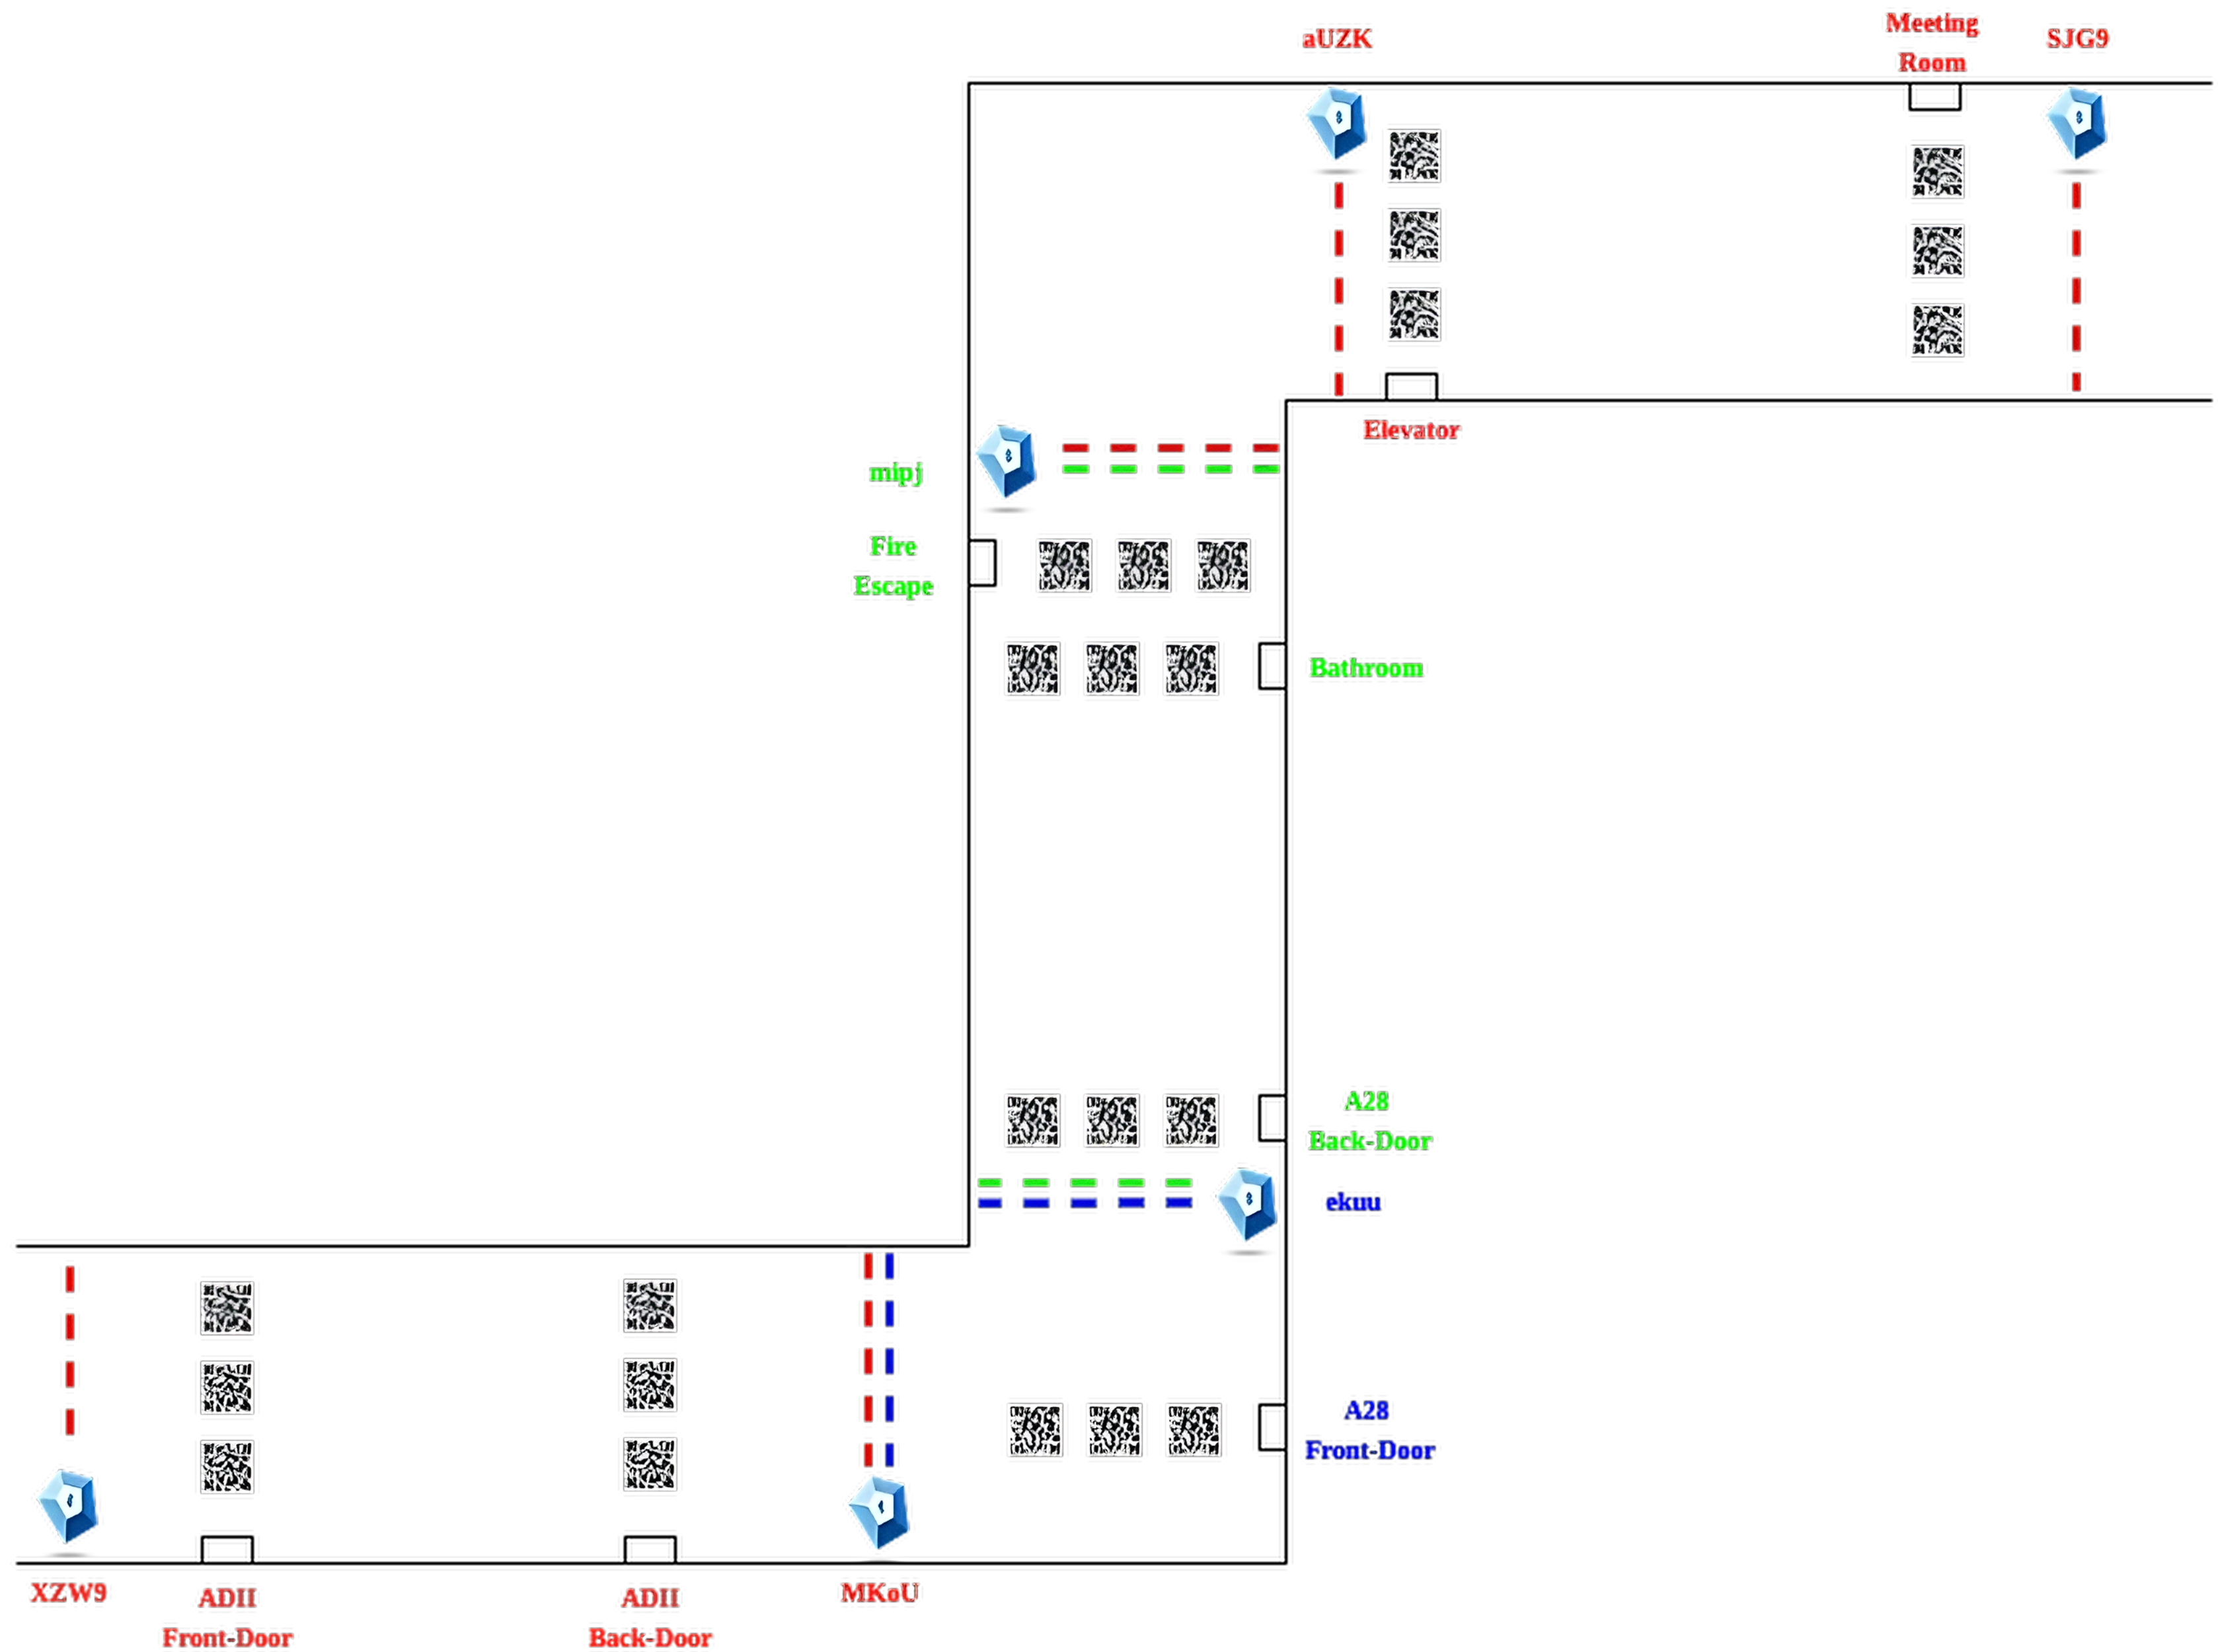
\includegraphics[scale = 0.12]{chapters/experimental_results/images/regions_mapping.png}
    \caption{Mapping of the regions and relative points of interest of the test area} 
    \label{fig:regions_mapping}
\end{figure*}
\noindent
Figure \ref{fig:regions_mapping} shows how the various initially introduced elements of the environment were mapped through the use of beacons and QR codes. This configuration was then placed into \textbf{JSON files} that are used by the application to be able to correctly execute the implemented detection algorithm.


\subsection{Application test}
A series of tests were conducted to evaluate the effectiveness and accuracy of our approach. They were performed using different smartphones to verify the application's behavior with various Android versions and hardware resources, ensuring its compatibility and proper functioning. The tests consisted in using the application while walking along the instrumented path (in both directions), simulating real usage scenarios. The smartphone must be positioned in parallel to the floor, to ensure that QR codes placed on the floor can be properly framed and scanned. On the other hand, if the user intends to search for a specific point of interest through a QR code located on a door, the smartphone should be held in a vertical position. Figure \ref{fig:application-test} illustrates an example of the test procedure with the correct positioning of the phone.

\begin{figure}[H]
    \centering
    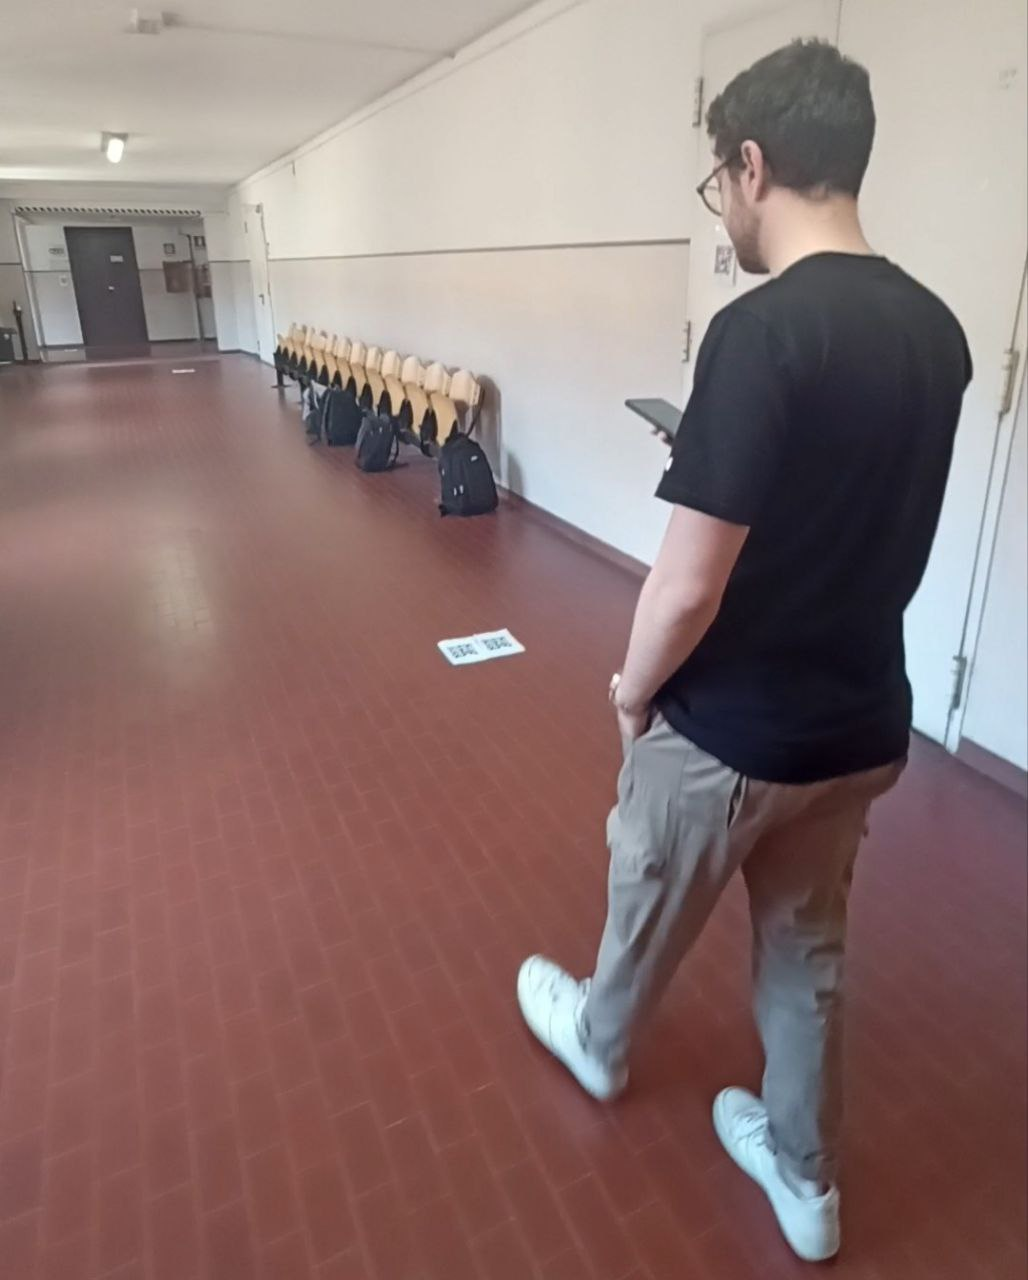
\includegraphics[width=0.8\columnwidth]{chapters/experimental_results/images/application_test.jpg}
    \caption{Final application tests}
    \label{fig:application-test}
\end{figure}

\subsubsection{Region change detection}
The evaluation focused on the application's ability to accurately detect transitions from one region to another. The application demonstrated the correct detection of region changes, with only sporadic instances of slight delay due to interference. In the majority of cases, the identification of new regions was performed accurately. The appropriate list of points of interest was provided to the users via the \textbf{TextToSpeech} \cite{android:text-to-speech-ref} functionality.

\subsubsection{Curve detection}
During the tests, we approached the curves along the path, and the application was evaluated on its capability to identify them and their direction (based on the previous region, which is always a pre-curve),  notifying users promptly. 
In most cases, the application demonstrated satisfactory performance in notifying users about curves, contributing to a smoother navigation experience.

\subsubsection{QR code detection}
The evaluation assessed the detection of QR codes placed on the ground and on the doors of points of interest. The application consistently and reliably detected floor QR codes while participants were walking, enabling the immediate delivery of audible notifications regarding nearby points of interest. Moreover, participants successfully scanned door QR codes, which allowed them to accurately determine the precise location of the points of interest.

\subsubsection{Application accessibility}
The conducted tests confirmed the application's compatibility with \textbf{Talkback} \cite{android:accessibility}, enabling visually impaired users to interact effectively with the application. 
These tests specifically focused on the different scenarios where user interaction is required. 

Additionally, \textbf{TextToSpeech} \cite{android:text-to-speech-ref} functionalities provide spoken announcements and instructions, eliminating the need for visually impaired users to rely on visual cues. In this way, visually impaired users will be able to use the application with ease.


\subsection{Limitations}
The main limitations of the adopted approach are the following:

\subsubsection{Infrastructure}
The indoor navigation assistant relies on the presence of a network of Bluetooth Low Energy (BLE) beacons and strategically placed QR codes. The effectiveness of the system is directly tied to the availability and maintenance of these infrastructure components. If the beacons or QR codes are damaged, removed, or not properly maintained, it can affect the accuracy and reliability of the navigation assistance.

\subsubsection{Coverage}
The system described is implemented in a specific building, and the infrastructure is deployed only in a section of that building. Therefore, the area covered by the system is limited to the instrumented section. Scaling up the system to cover larger buildings or multiple buildings would require additional configuration. The deployment of the BLE beacons and QR codes requires manual effort and careful placement. This process can be time-consuming and resource-intensive, especially for larger indoor environments. 

\subsubsection{Accuracy}
The accuracy of the localization and navigation functionalities using BLE beacons can be affected by signal interference or environmental factors such as walls, obstacles, or electromagnetic interference. Interference from other devices or signal propagation limitations within the building can result in inaccuracies in determining the user's location or detecting region switches. 
The system's performance and accuracy may also change when applied to indoor environments with varying layouts, sizes, or infrastructure configurations. 

\subsubsection{Additional functionalities}
The system lacks more advanced features found in commercial indoor navigation solutions. For instance, the application does not provide specific directions or routes to individual destinations within the building.
By incorporating advanced localization techniques such as \textbf{triangulation} or \textbf{fingerprinting} \cite{10.1145/3058555.3058560}, it would be possible to introduce additional functionalities like point-to-point navigation and improve the overall reliability of the application.
Moreover, through the adoption of more complex approaches, the possibility of incorporating supplementary features, such as detecting intersections, as well as managing indoor open areas, could be achieved.

Currently, the application loads information from JSON files. While this approach is very simple and allows for flexibility in managing the data, alternative methods could be explored. For instance, using a cloud-based database solution like \textbf{Firebase} \cite{firebase} could provide real-time updates and seamless synchronization of data across multiple devices.



\section{Conclusions}
In conclusion, this paper addresses the challenge of indoor-assisted navigation for individuals who are blind or visually impaired by proposing a hybrid approach utilizing Bluetooth Low Energy (BLE) beacons and QR codes. 

The developed application was tested in a section of the main building at the School of Engineering, University of Pisa, and the results were satisfactory. The application successfully guided users along the designated path, accurately detecting region switches, nearby points of interest, and incoming curves, while demonstrating good responsiveness and accuracy in providing navigation assistance.

However, several limitations need to be taken into account. Ensuring the availability of Bluetooth Low Energy (BLE) beacons and QR codes is crucial, requiring regular maintenance and upkeep. Scaling up the system to cover larger areas necessitates additional configuration and environmental instrumentation. To enhance accuracy, it is important to overcome signal interference and adapt to different indoor environments. Moreover, incorporating advanced localization techniques and introducing features like point-to-point navigation would greatly improve functionality. Exploring alternative data loading methods, such as a cloud-based database solution, could provide real-time updates and seamless synchronization across devices.

In summary, the proposed hybrid approach combining BLE beacons and QR codes has proven to be effective in assisting individuals with visual impairments in navigating indoor environments. The results obtained from testing demonstrate the feasibility and potential of this approach. However, it is important to consider the mentioned issues and the possibility of incorporating additional functionalities to enhance the overall user experience.
\label{sec:conclusion}


% References
\hypersetup{
    urlcolor=black
}
\nocite{*}
\printbibliography


\end{multicols*}

\end{document}
